\chapter{Introduction}
\label{chap:Introduction}

Optical music recognition (OMR) is the task of extracting semantic information from scans and photos of sheet music. It is a subfield of computer vision, however, traditional computer vision methods are struggling with it unsuccessfully. Especially in the subfield of handwritten music recognition (HMR), where the large variability of handwriting styles poses a great challenge for any handcrafted recognition system. For this reason, recent advances in the field have been made mainly due to the adoption of deep learning. OMR is also a relatively niche field, studied by a minority of researchers and as such does not have the resources to produce large annotated datasets (compared to speech recognition, natural language translation or text recognition). Existing datasets are either small, or designed for a simpler problem (like staff removal). This poses a challenge to training large neural networks and further application of deep learning. There is, however, a relative abundance of unlabeled data.

The largest dataset of handwritten music sheets is CVC-MUSCIMA, containing 1000 pages (\cite{CvcMuscima}). The dataset was designed for writer identification and staff removal, therefore it can not be used to learn, for example, object detection. A subset of 140 pages has been labouriously annotated by \cite{MuscimaPP} to form the MUSCIMA++ dataset. This dataset can be used to train models for many tasks, since the annotation scheme (Music Notation Graph) is very versatile, however there are still 860 unannotated pages of the original CVC-MUSCIMA dataset, that are not used during such a training. This situation is exactly what semi-supervised learning is designed to deal with.

Semi-supervised learning (SSL) is a collection of methods, that aim to incorporate the unlabeled data during training to produce a more performant model. Many of these methods are designed for classification problems. Unfortunately, we explore SSL in the context of semantic segmentation and this lets us utilize only generative methods of SSL. We do not focus on traditional classification, because it is not a scheme applicable for processing entire pages of music. It can only classify already detected symbols. Moreover, semantic segmentation is able to classify symbols of rather extreme dimensions and varying shapes (e.g.\@ slurs and beams\footnote{slurs and beams are elongated symbols of music notation}) that cannot be realistically cropped and classified in a traditional setting. Semantic segmentation is also used as a basis for object detection, which is the most important step of every music recognition pipeline.

It has been shown that the U-Net architecture yields the best results for semantic segmentation of musical symbols (\cite{UNet}, \cite{PachaBaseline}). The architecture is also similar to a variational autoencoder, which is at the heart of generative semi-supervised learning. This motivates us to use a U-Net for our SSL exploration. The U-Net architecture was designed specifically for semantic segmentation and the presence of skip connections and the fact of being fully convolutional are direct consequences of this intention. These same properties, however, make it difficult to use for semi-supervised learning. Skip connections prevent the use of this architecture for unsupervised learning (as a generative model) and the fully convolutional property complicates interpretability of the latent space.

We have designed a novel scheme for training a U-Net model that sidesteps these complications and lets us train the model in a semi-supervised way. We consider this scheme to be the main contribution of this thesis.

Our scheme pivots around the idea of masking out parts of the input image and training the network to reconstruct the full image. This allows us to train the model like an autoencoder and have it learn abstract features, despite having skip connections between the encoder and the decoder. Figure \ref{fig:Reconstructions} shows a reconstructed image, where generated stafflines and stems are clearly visible.

\begin{figure}[ht]
    \centering
    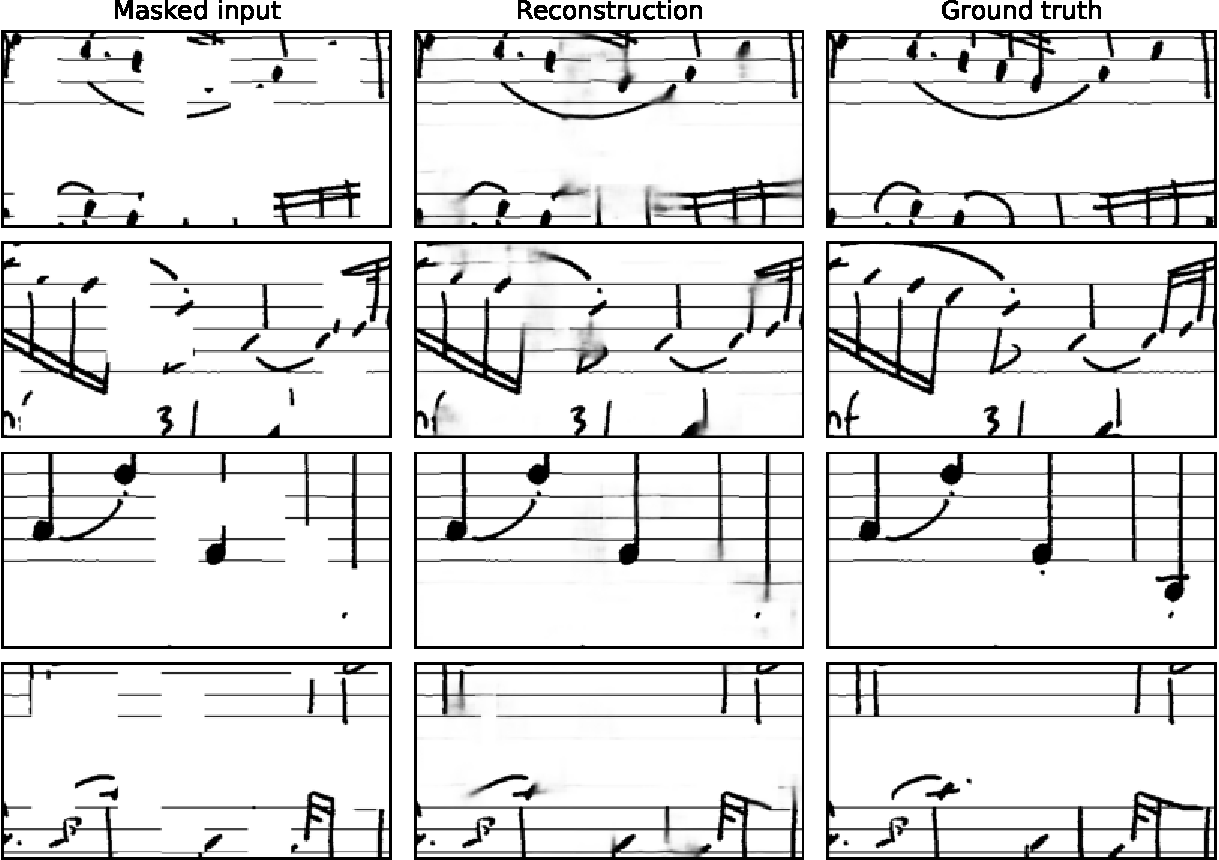
\includegraphics[width=145mm]{../../figures/06-noise/reconstructions.pdf}
    \caption{Our training scheme manages to train a U-Net architecture in an unsupervised manner to produce reconstructions of masked images. Each row is an example of a performed reconstruction (middle column), together with the input and expected output (side columns). We can see that stafflines are reconstructed very well, whereas more complicated symbols tend to get blurred out.}
    \label{fig:Reconstructions}
\end{figure}

Most of our experiments focus on notehead segmentation, because noteheads are an ideal symbol for this kind of experimentation. They are abundant in the input images, they are the most important symbol semantically, and they have great variability in terms of appearance (handwritten noteheads).

We train the model in the context of three experiments and compare it against a corresponding supervised baseline. The model prediction is evaluated using pixelwise F1 score, as it aggregates both precision and recall into a single number. Performing the evaluation pixelwise lets us compare the model to the baseline with minimal added complexity (e.g.\@ bounding box detection) and thus provide direct feedback on the only property varied -- the amount of unlabeled data.

All three experiments suggest, that training a U-Net in this semi-supervised scheme acts as regularization and helps stabilize the training. Unfortunately, we did not manage to surpass the supervised baseline, we only got the same performance. We belive that training the reconstruction with \emph{pixelwise binary cross entropy} loss function causes the model to produce fuzzy reconstructions and to learn representations that are not useful for improving segmentation performance. This may be because there are many possible reconstructions of a masked area, and the model learns to reconstruct their fuzzy average, instead of picking one and making a good-looking reconstruction. We belive that adding a smarter loss function, such as a discriminator network, could lead to improvements. We plan to explore this idea in a future work.

Primary contributions in this thesis are:

\begin{itemize}
    \item Modification of the U-Net architecture for simultaneous segmentation and reconstruction.
    \item Unsupervised training scheme for the architecture based on reconstructions of masked patches.
    \item Thorough exploration of relevant hyperparameters.
    \item Detailed experiments, designed to assess the viability of this model in the semi-supervised setting.
\end{itemize}

Code for the model and all experiments is available in a GitHub repository at \url{https://github.com/Jirka-Mayer/MasterThesis}.


\section{Thesis Outline}

\paragraph*{Chapter \ref{chap:Introduction}} This chapter is a condensed overview of the entire thesis, starting with the context and our motivation, describing the architecture and experiments and closing of by taking about possible future work.

\paragraph*{Chapter \ref{chap:RelatedWork}} This chapter is a short overview of the most influential articles for this thesis. It introduces the U-Net architecture and describes it in the context of music recognition. It concludes by highlighting the abilities of semi-supervised generative models.

\paragraph*{Chapter \ref{chap:OMR}} This chapter is a brief overview of the field of optical music recognition. It describes the transition from traditional approaches to deep learning, lays out the currently accepted recognition pipeline, and ends by introducing all of the datasets used in this thesis.

\paragraph*{Chapter \ref{chap:SemisupervisedLearning}} This chapter is an overview of semi-supervised methods, grouped into their respective categories. More attention is given to generative semi-supervised methods, which are explored in the second half of the chapter.

\paragraph*{Chapter \ref{chap:Methodology}} This chapter contains detailed description of the proposed architecture and the preparation of its training data. It also talks about the chosen evaluation metrics.

\paragraph*{Chapter \ref{chap:ExperimentsAndResults}} This is the core chapter of this thesis. It starts with an overview of relevant hyperparameters and experiments we did to set their default values. The last three sections describe three major experiments. The first two assess the viability of our model in the semi-supervised setting (Section \ref{sec:SemisupervisedImprovements} and Section \ref{sec:UtilizingCvcMuscima}). The last experiment is a mixture of transfer learning and semi-supervised learning (Section \ref{sec:KnowledgeTransfer}), where we attempt to learn handwritten music segmentation from printed ground-truth music.
